\documentclass[tikz,border=8pt]{standalone}
\usepackage{amsmath}
\usepackage{tikz}
\usetikzlibrary{calc,patterns,arrows.meta}

\begin{document}
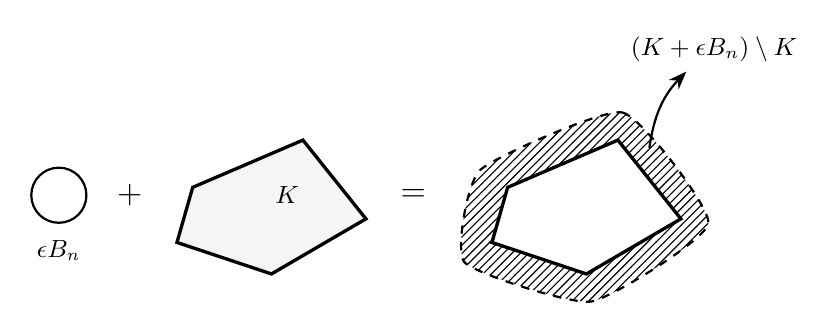
\begin{tikzpicture}[scale=1, every node/.style={font=\small}]

  % 参数
  \def\eps{0.35}    % 视觉上的 epsilon(小圆和底部矩形高度)
  \def\xsep{4.0}    % 左中右块水平间距
  \def\tension{0.3} % smooth cycle 张力

  % ---- 左侧: epsilon B_n ----
  \begin{scope}[shift={(-3.5,0)}]
    \draw[thick] (0,0) circle[radius=\eps];
    \node at (0,-\eps-0.35) {$\epsilon B_n$};
  \end{scope}

  % ---- 中间: 原始凸体 K(中心) ----
  \coordinate (K1) at (-1.8,0.1);
  \coordinate (K2) at (-0.4,0.7);
  \coordinate (K3) at (0.4,-0.3);
  \coordinate (K4) at (-0.8,-1.0);
  \coordinate (K5) at (-2.0,-0.6);

  \begin{scope}[shift={(0,0)}]
    \filldraw[fill=gray!8, draw=black, very thick]
      (K1) -- (K2) -- (K3) -- (K4) -- (K5) -- cycle;
    \node at (-0.6,0) {$K$};
  \end{scope}

  % 等号符号(放在中间上方)
  \node at (-2.6,0) {\large +};
  \node at (1.0,0) {\large =};

  % ---- 右侧: 平移后的 K (RK) 与其圆润 Minkowski 膨胀外壳 ----
  % 将中间的 K 平移到右侧作为内边界 RK
  \coordinate (RK1) at ($ (K1) + (\xsep,0) $);
  \coordinate (RK2) at ($ (K2) + (\xsep,0) $);
  \coordinate (RK3) at ($ (K3) + (\xsep,0) $);
  \coordinate (RK4) at ($ (K4) + (\xsep,0) $);
  \coordinate (RK5) at ($ (K5) + (\xsep,0) $);

  % 手工调节的外扩顶点(基于 RK 顶点的局部偏移,视觉上近似 Minkowski 膨胀)
  \coordinate (OK1) at ($(RK1)+(-\eps,0.22)$);
  \coordinate (OK2) at ($(RK2)+(0.06,\eps)$);
  \coordinate (OK3) at ($(RK3)+(\eps,-0.06)$);
  \coordinate (OK4) at ($(RK4)+(0.06,-\eps)$);
  \coordinate (OK5) at ($(RK5)+(-\eps,-0.25)$);

  % 在右侧绘制外壳(平滑闭合)并填充差集
  \begin{scope}[shift={(0,0)}]
    % 外壳平滑填充(先填外壳)
    \fill[pattern=north east lines, pattern color=black]
      plot[smooth cycle, tension=\tension] coordinates { (OK1) (OK2) (OK3) (OK4) (OK5) };
    % 覆盖内核 (白色) 以表现差集
    \fill[white] (RK1) -- (RK2) -- (RK3) -- (RK4) -- (RK5) -- cycle;
    % 边界:外壳(虚线)与内核(实线)
    \draw[black, thick, dashed] plot[smooth cycle, tension=\tension] coordinates { (OK1) (OK2) (OK3) (OK4) (OK5) };
    \draw[black, very thick] (RK1) -- (RK2) -- (RK3) -- (RK4) -- (RK5) -- cycle;
    % 标签
    % \node at ($ (RK2) + (-0.6,0.9)$) {$K+\epsilon B_n$};
  \end{scope}

  % 箭头与标注:指向右侧阴影壳层
\node[above right,xshift=4pt,yshift=2pt] (mylbl) at ($( \xsep-0.5,1.5)$) {$(K+\epsilon B_n)\setminus K$};
\draw[->, >=Stealth, thick] ($( \xsep,0.6)$) to[bend left=18] (mylbl);

  % % ---- 底部:高度为 epsilon 的长方形,标注 perimeter of K ----
  % \begin{scope}[shift={(0,-2.2)}]
  %   \def\W{5.2}
  %   \draw[thick] (-\W/2,0) rectangle (\W/2,\eps);
  %   \node at (0,-0.4) {\textbf{perimeter of K}};
  %   \draw[<->] (\W/2+0.2,0) -- (\W/2+0.2,\eps) node[midway,right] {$\epsilon$};
  % \end{scope}

\end{tikzpicture}
\end{document}
